\documentclass[devoir3.tex]{subfiles}

\begin{document}

\section*{Question 4}
Supposez que vous ayez un damier \(n \times n\) et un jeton. Vous devez déplacer
le jeton depuis le bord inferieur du damier vers le bord supérieur, en respectant la règle suivante. À chaque étape, vous pouvez placer le jeton sur l’un des trois carrés suivants

\begin{itemize}
	\item le carré qui est juste au dessus,
	\item le carré qui est une position plus haut et une position plus à gauche (à condition que le jeton ne soit pas déjà dans la colonne la plus à gauche),
	\item le carré qui est une position plus haut et une position plus à droite (à condition que le jeton ne soit pas déjà dans la colonne la plus à droite).
\end{itemize}

\begin{figure}[H]
	\centering
	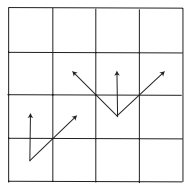
\includegraphics[width=6cm]{fig2}
	\caption{Graphe}
	\label{fig:fig2}   
\end{figure}

La figure \ref{fig:fig2} illustre les déplacements valides à partir de deux positions dans un damier de dimension \(4 \times 4\). \\

Chaque fois que vous vous déplacez du carré \(x = (i, j)\) au carré \(y \in \lbrace (i-1,j-1),(i-1,j),(i-1,j+1) \rbrace \), vous recevez \(p(x, y)\) dollars. On vous donne \(p(x, y)\) pour toutes les paires \((x, y)\) correspondant à un déplacement licite de \(x\) à \(y\). \(p(x, y)\) \textbf{n’est pas forcément positif}. \\

Donner un algorithme efficace de programmation dynamique pour déterminer le montant maximum que vous pouvez empocher. Votre algorithme peut partir de n’importe quel carré du bord inférieur et arriver sur n’importe quel carré du bord supérieur pour maximiser le montant collecté au cours du trajet. \\

Expliquez comment vous pouvez optimiser l’espace mémoire et évaluez le temps d’exécution et l’espace mémoire de votre algorithme. \\

\end{document}
